\preparagraphspacing{}
\section*{Change Descriptors}
\label{sec:chdescs}

What they are
What they're for, abstractly (short)
History, better than GEOM, JBD
How to generate the correct chdescs
What they contain
How they move around
How we use them (transformations, applications)
Relationship to consistency models
User-level chdescs
Chdesc challenges - memory pressure, time, circularity

In contrast with traditional systems, where changes to filesystem data are
accomplished by changing in-memory copies of the disk blocks and marking the
block as needing to be written to disk (thus losing all record of what was
changed), every change to filesystem data in the KudOS file server effects a
corresponding ``change descriptor'' that describes what was changed. Change
descriptors (``chdescs'' for short) allow individual changed to be undone and
redone (``rolled back'' and ``rolled forward''), as well as allowing a
dependency graph to be created describing which changes depend on which other
changes already being written to disk. XXX(These two capabilities allow any
module in the system to inspect and even modify the changes that other modules
are making.)

\begin{figure}
\begin{verbatim}
struct chdesc {
    BD_t * owner;
    bdesc_t * block;
    enum {BIT, BYTE, NOOP} type;
    union {
        struct {
            uint16_t offset;
            uint32_t xor;
        } bit;
        struct {
            uint16_t offset, length;
            uint8_t * data;
        } byte;
    };
    struct chdesc * dependencies[];
};
\end{verbatim}
\vspace{-10pt}
\caption{\label{fig:chdesc} Change descriptor structure}
\end{figure}

{\bf This section refers to LFS before it is defined.}

The ability to revert and re-apply chdescs is inspired by the ``soft updates''
system in BSD's FFS~\cite{ganger00soft}, but it is generalized so that it is not
specific to any particular filesystem. A chdesc can describe a change as small
as a single bit, or as large as a whole disk block. Soft updates, journalling,
and many application-specific consistency models all correspond to different
change descriptor arrangements. Block data is almost secondary to the chdescs
from the point of view of the file system server -- chdescs are what really move
around in the system. This concept allows some interesting configurations of
modules as well as very simple implementations of traditionally complicated
features. For instance, journalling is implemented as a single block device
module, and it can automatically add journalling -- even metadata-only
journalling -- to {\it any} LFS filesystem. Other block device layering systems,
like GEOM~\cite{geom}, would need special hooks into filesystem code in order to
get the necessary hints (i.e. what is metadata and what is not) to do
metadata-only journalling. Change descriptors and the LFS interface division
allow us to do this automatically.

\begin{figure}[b]
  \centering
  \includegraphics[width=80pt]{fig/whatevs_3}
  \caption{\label{fig:softupdates} Modeling a soft updates operation using
  change descriptors.}{Four change descriptors can describe the dependencies
  for allocating a new indirect block and attaching it to file. Writing the
  new block pointer to an inode ($C$) depends on initializing the block ($A$)
  and updating the free block map. ($B$) Attaching the indirect block ($D$)
  depends on its allocation ($C$).
}
\end{figure}

\begin{figure}
  \centering
  \includegraphics[width=\columnwidth]{fig/whatevs_2}
  \caption{\label{fig:journal} Journal change descriptor graph.}{The original
  four change descriptors from Figure~\ref{fig:softupdates} are made to depend
  on a journal commit record, which depends on copies ($A_j$, $B_j$, $C_j$, and
  $D_j$) of the original change descriptors being written to the journal. A
  commit record cancellation depends on the original change descriptors. The
  empty circles are ``NOOP'' change descriptors which have no associated block
  data.}
\end{figure}

For many complex operations, like RAID or journalling, the chdesc graph is
changed in specific ways which can be broken down into sequences of simple graph
transformations. For example, in the (mirroring) RAID module it is necessary to
duplicate a change descriptor, including all its dependents and dependencies. We
expect that after implementing a relatively small number of more complex modules
(we have only implemented the two mentioned), we will have seen similarities in
many of the transformations and will have built up a fairly complete library of
common transformation functions.

\begin{figure}
  \centering
  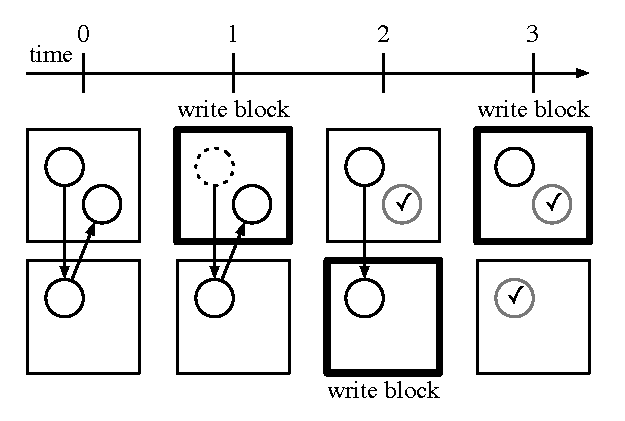
\includegraphics[width=200pt]{rollback_sequence}
  \caption{\label{fig:rollback} Rolling back change descriptors.}{Although no
  cycles are allowed in change descriptor graphs, cycles can exist at the block
  level which require some change descriptors to be rolled back in order to
  write the blocks. Here the squares are blocks, and dotted circles are rolled
  back change descriptors.}
\end{figure}
